% PsychoPy tutorial
% Ariel Rokem
% License:CC(http://creativecommons.org/licenses/by-nc-sa/3.0/)

\documentclass{beamer}

\usepackage{ulem}
\usepackage{listings,bera}

\usetheme{PaloAlto}
\beamertemplatenavigationsymbolsempty

\definecolor{fore}{RGB}{0,20,30}
\definecolor{back}{RGB}{255,255,255}
\definecolor{title}{RGB}{255,255,255}


\setbeamercolor{titlelike}{fg=title}
\setbeamercolor{normal text}{fg=fore,bg=back}
\definecolor{keywords}{RGB}{255,0,90}
\definecolor{comments}{RGB}{60,179,113}
\definecolor{strings}{RGB}{120,120,0}

\lstset{language=Python,
keywordstyle=\color{keywords},
commentstyle=\color{comments}\emph,
stringstyle=\color{strings}}

\title[nitime]{\tt{nitime}}
\subtitle
{Time-series analysis for fMRI data}

\author[Ariel Rokem] % (optional, use only with lots of authors)
{Ariel Rokem}
\date{June 3rd, 2011}
\institute[University of California, Berkeley]
{University of California, Berkeley}

\pgfdeclareimage[height=1.5cm]{ucb-logo}{figures/ucb_logo}
% put nipy logo in bottom left
\pgfdeclareimage[height=1.5cm]{nipper}{figures/nipper}
\setbeamertemplate{sidebar left}{
   \rlap{\hskip0.1cm%
     {\pgfuseimage{ucb-logo}}}
    \vfill%
   \rlap{\hskip0.1cm%
     {\pgfuseimage{nipper}}}%
   \vskip2pt%
   \llap{\usebeamertemplate***{navigation symbols}\hskip0.1cm}%
   \vskip2pt%
}

\begin{document}

%Title page:
\begin{frame}
  \titlepage
\end{frame}

\begin{frame}
\frametitle{The wiring diagram}
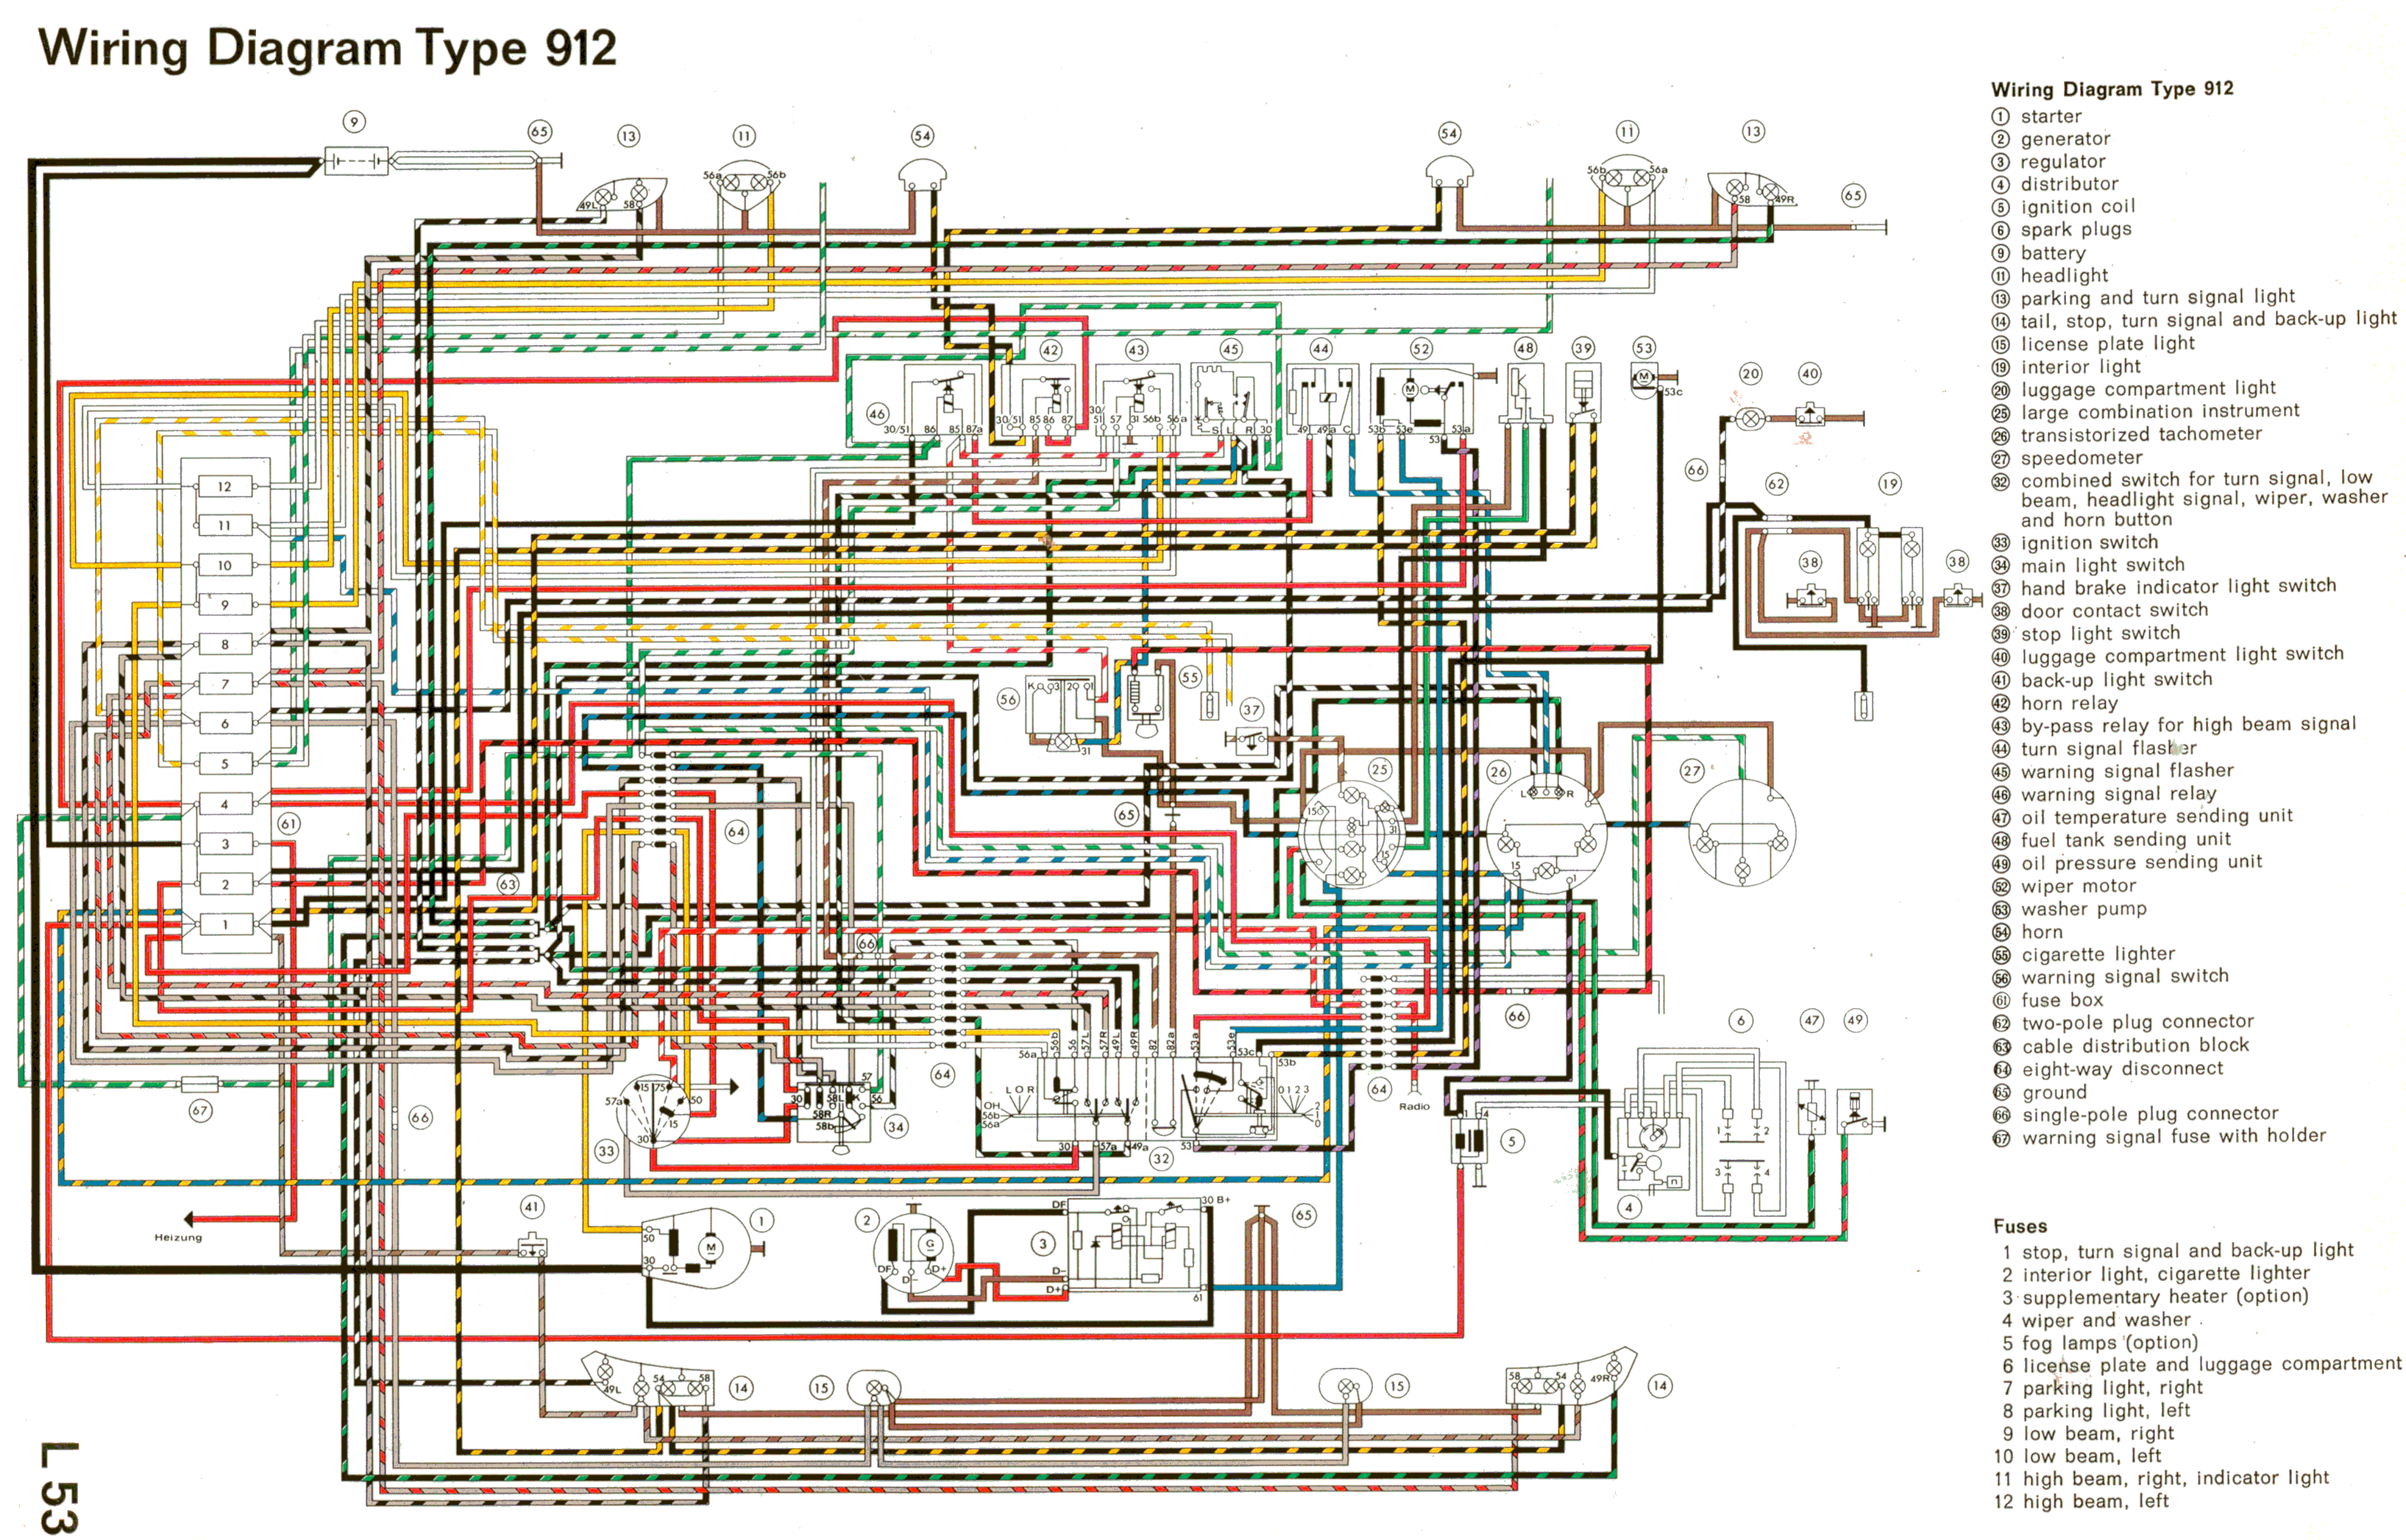
\includegraphics[height=5.7cm]{figures/wiring}
\end{frame}

\begin{frame}
\frametitle{The wiring diagram}
\includegraphics[height=5.7cm]{figures/felleman1}
\end{frame}

\begin{frame}
\frametitle{The wiring diagram}
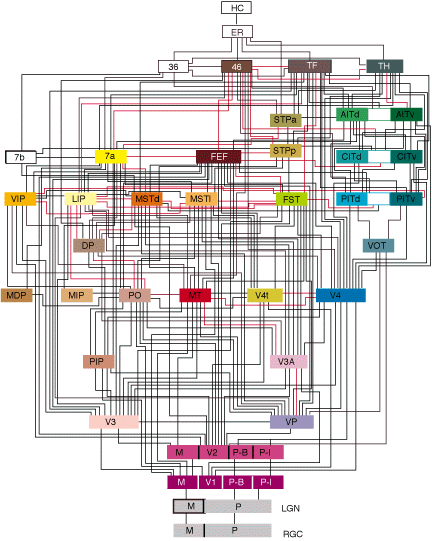
\includegraphics[height=5.7cm]{figures/felleman2}
\end{frame}

\begin{frame}
\frametitle{Task-specific networks}
  One of the goals of contemporary neuroscience is to delineate task-specific
  networks in the brain
\end{frame}

\begin{frame}
\frametitle{Time-series in fMRI data}
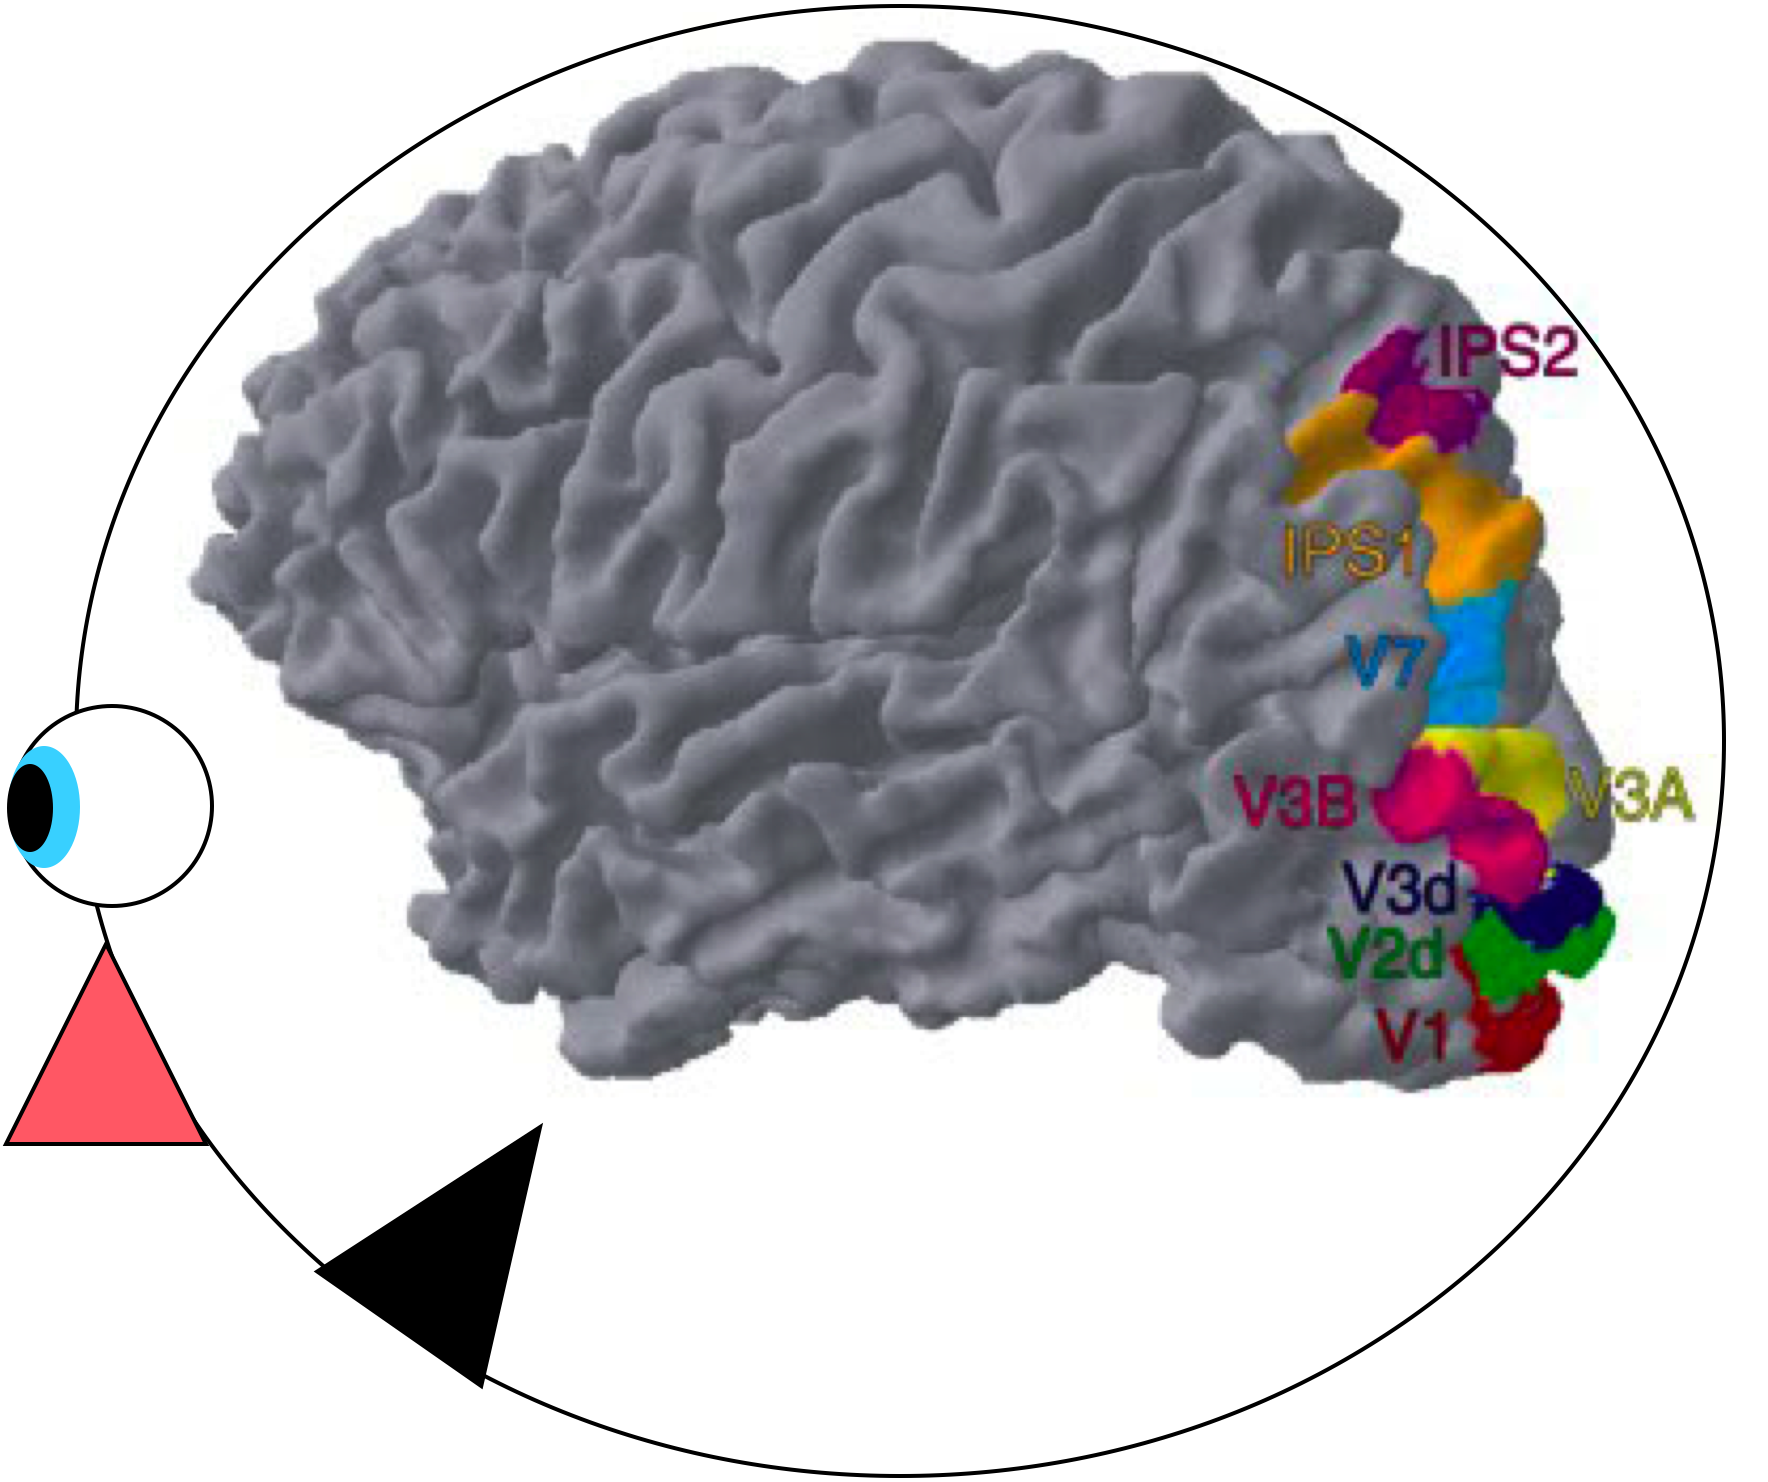
\includegraphics[height=5.7cm]{figures/brain_w_head}
\end{frame}

\begin{frame}
\frametitle{Time-series in fMRI data}
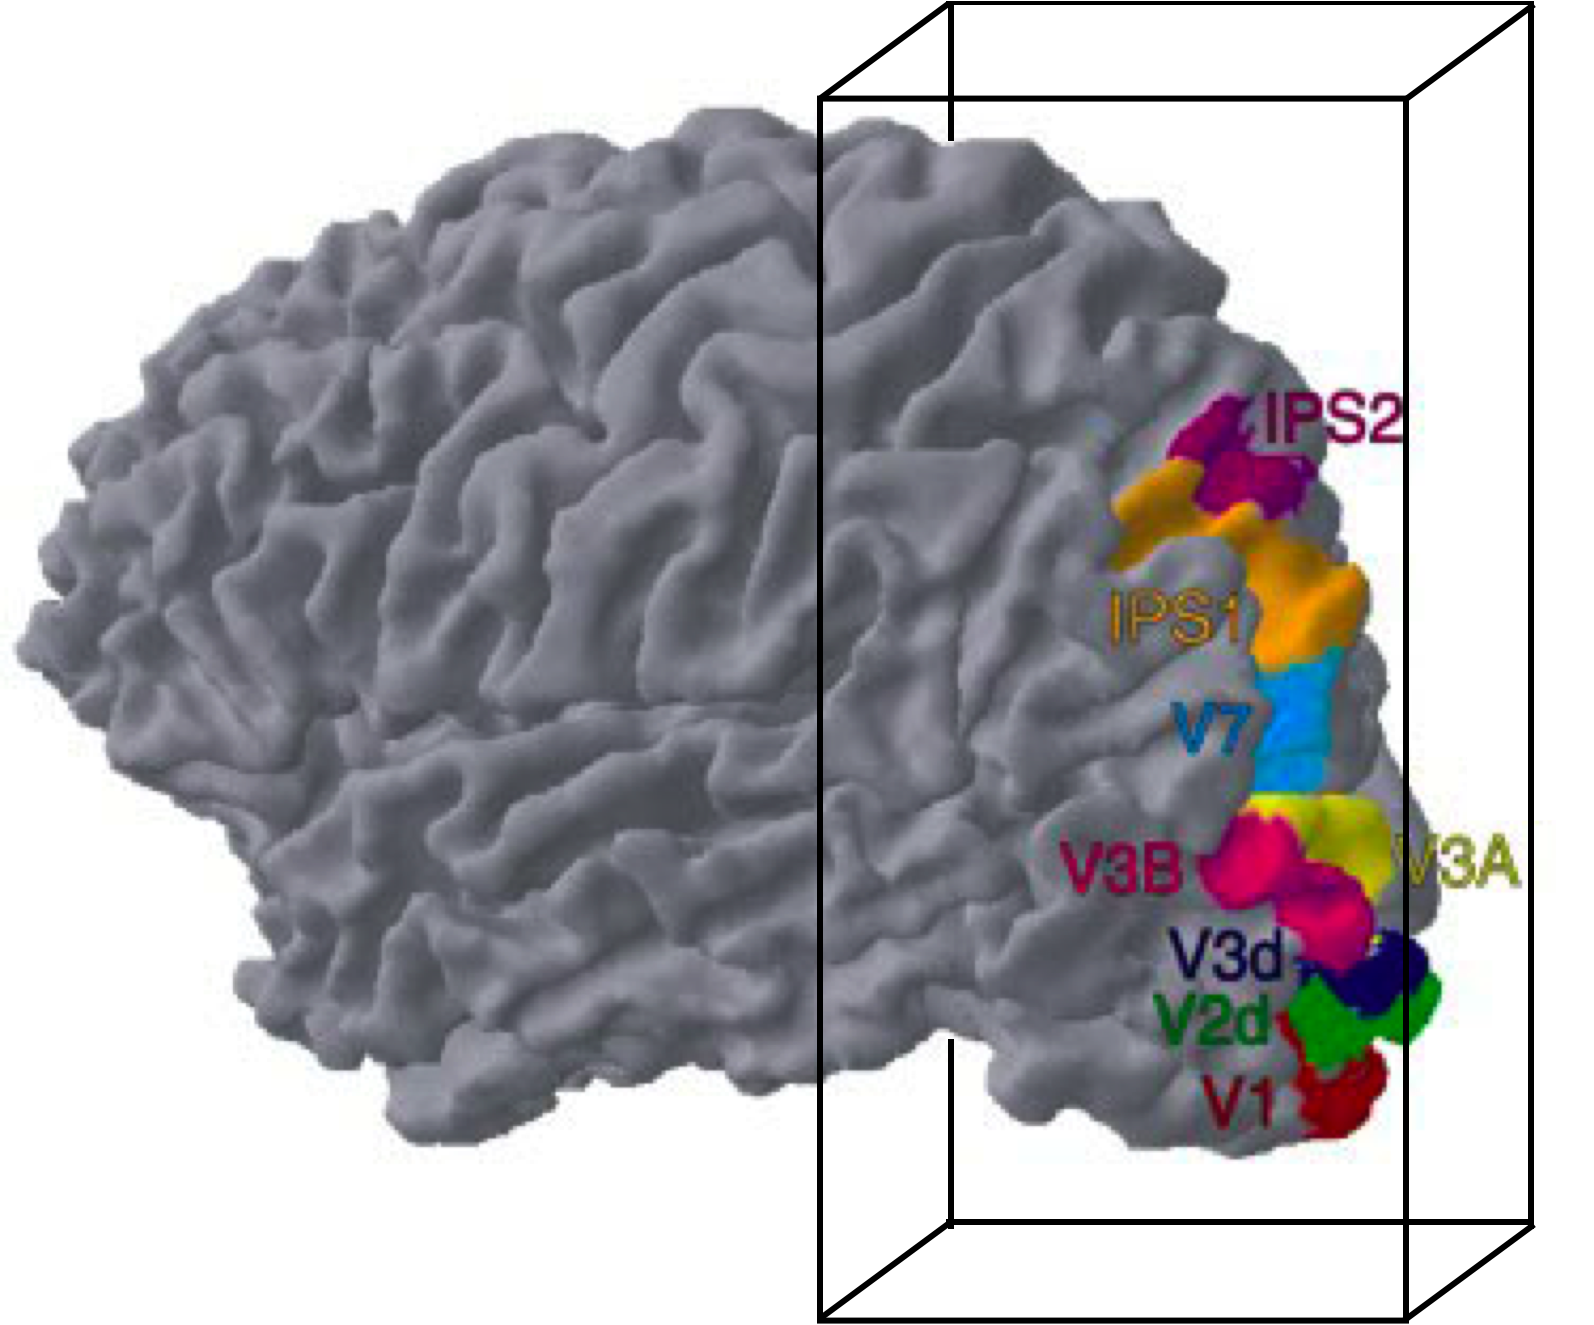
\includegraphics[height=5.7cm]{figures/brain_w_acquisition_vol}
\end{frame}

\begin{frame}
\frametitle{Time-series in fMRI data}
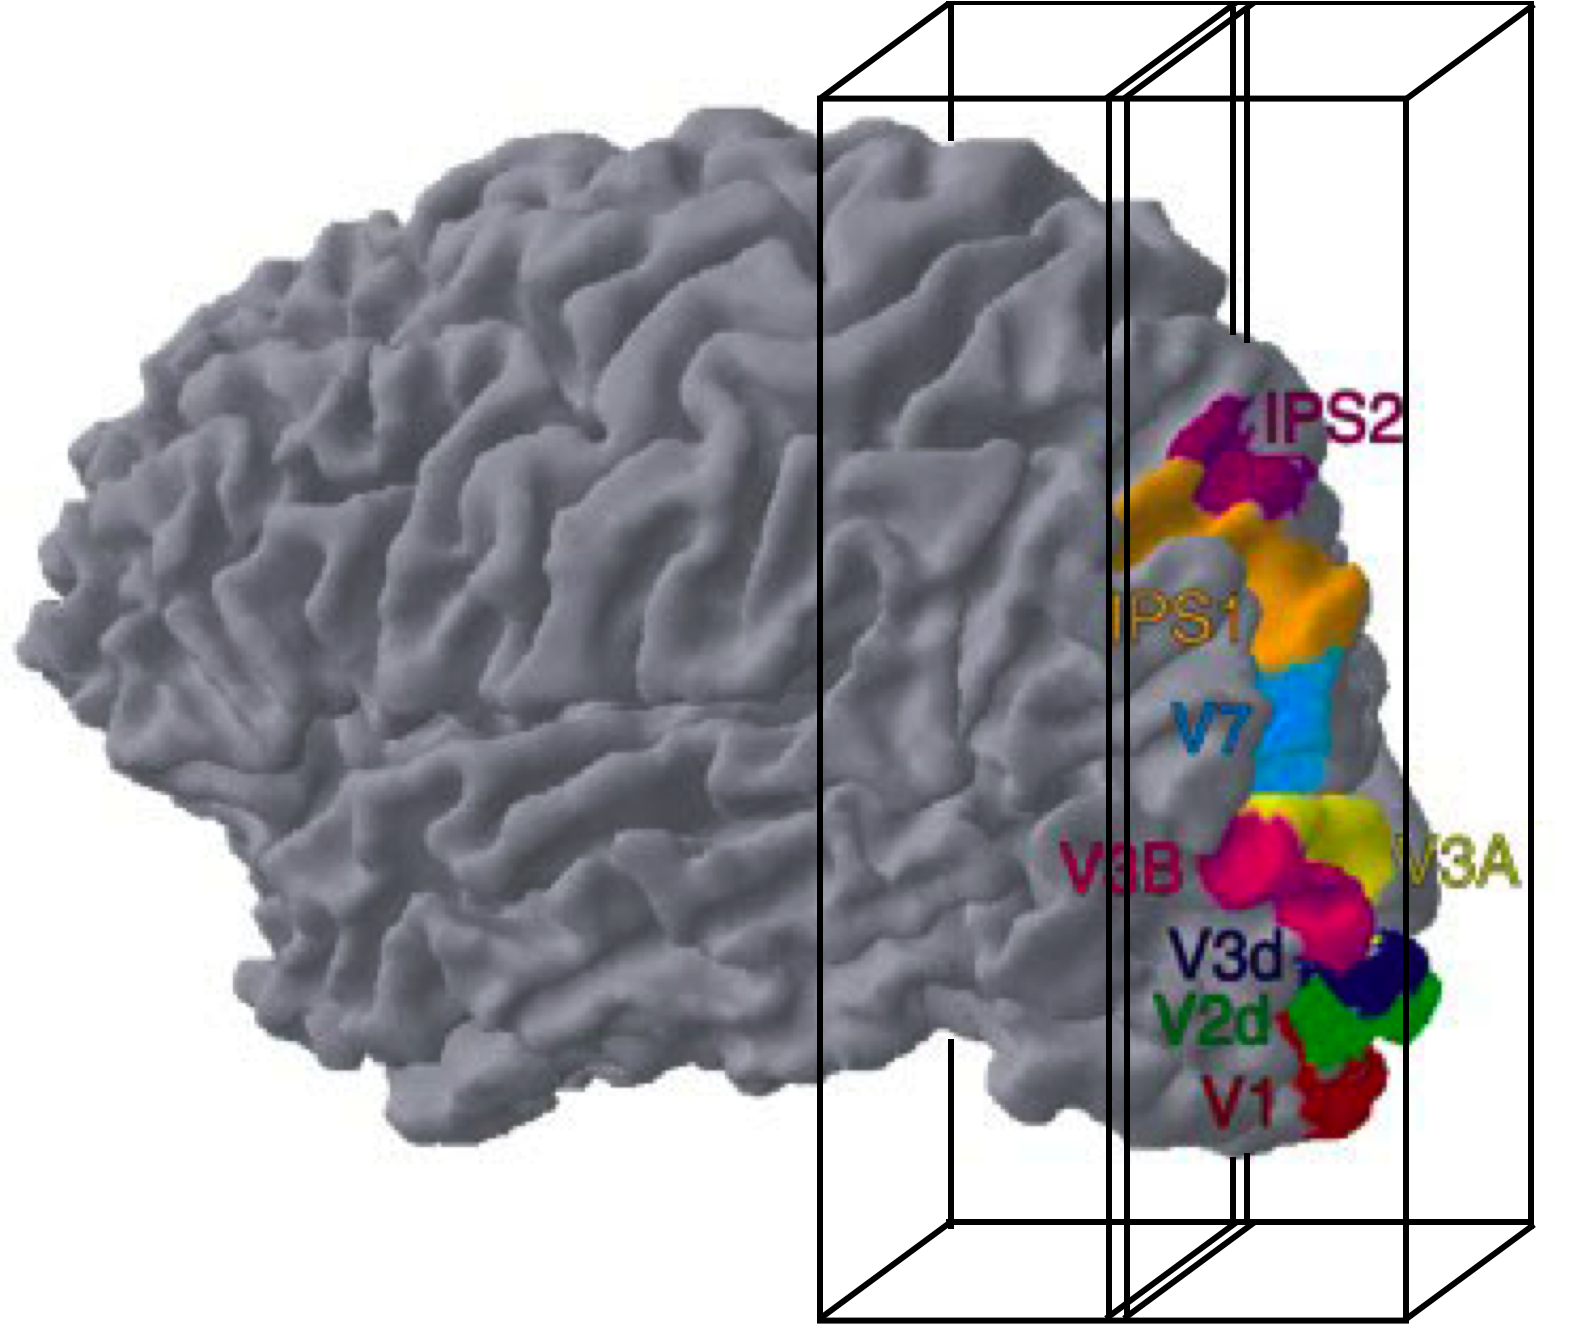
\includegraphics[height=5.7cm]{figures/brain_w_acquisition_vol_n_slice}
\end{frame}

\begin{frame}
\frametitle{Time-series in fMRI data}
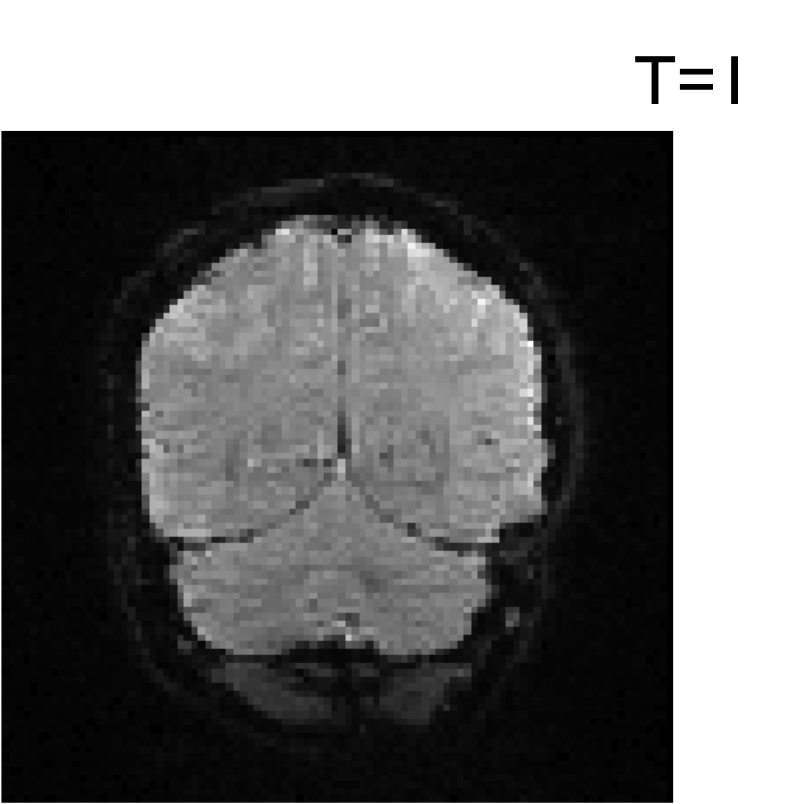
\includegraphics[height=5.7cm]{figures/t1}
\end{frame}

\begin{frame}
\frametitle{Time-series in fMRI data}
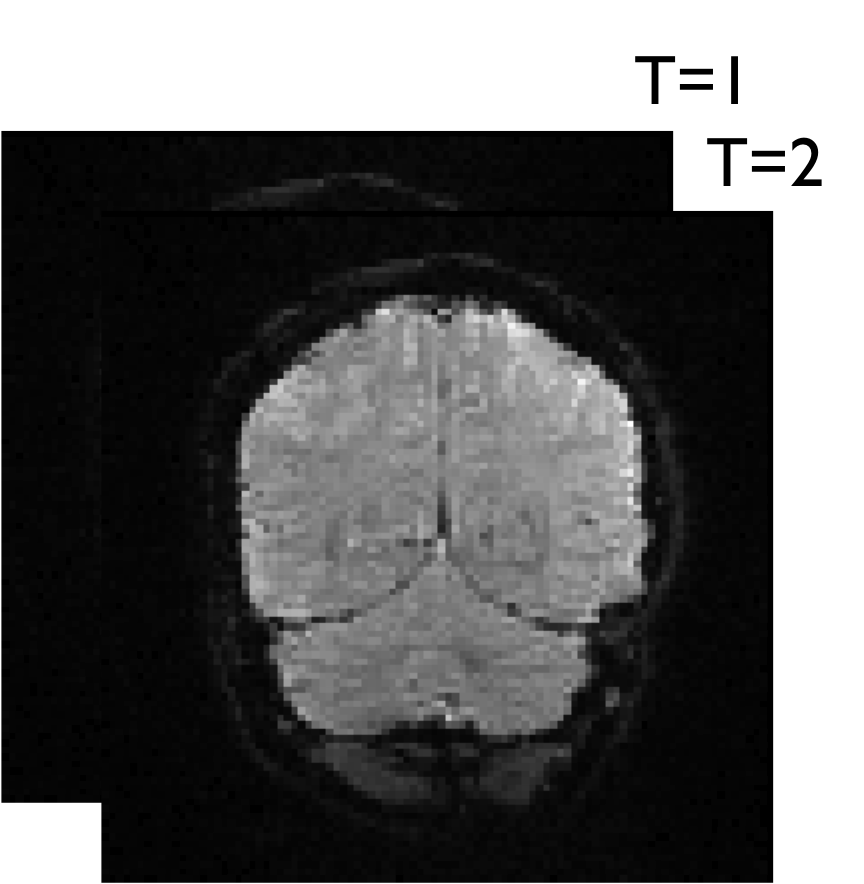
\includegraphics[height=5.7cm]{figures/t1_2}
\end{frame}

\begin{frame}
\frametitle{Time-series in fMRI data}
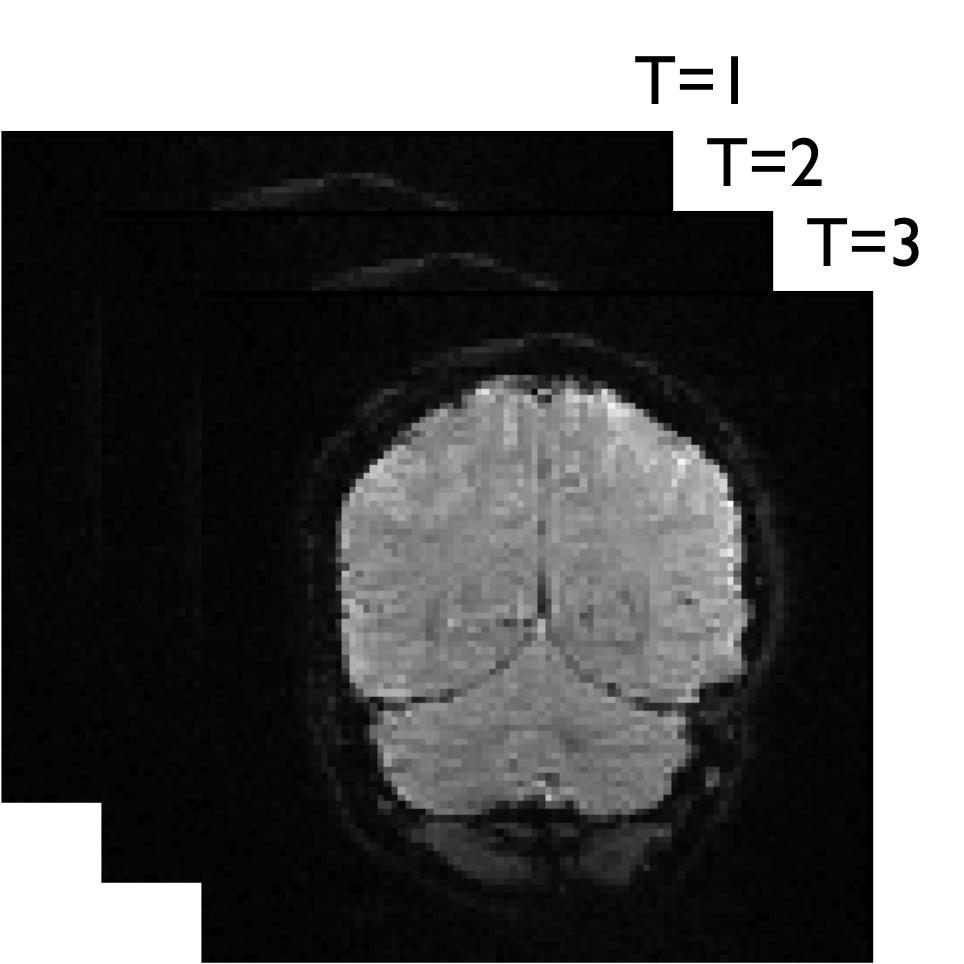
\includegraphics[height=5.7cm]{figures/t1_2_3}
\end{frame}

\begin{frame}
\frametitle{Time-series in fMRI data}
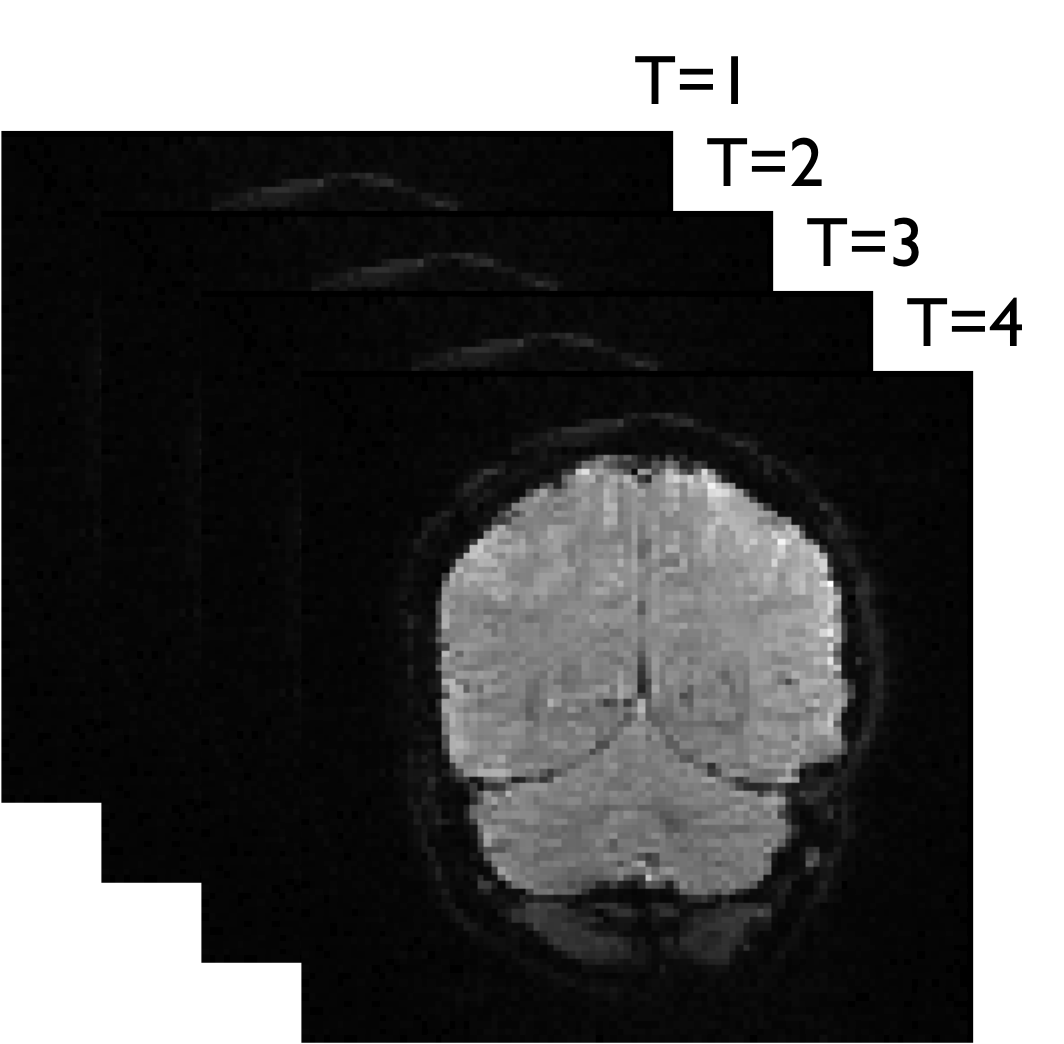
\includegraphics[height=5.7cm]{figures/t1_2_3_4}
\end{frame}

\begin{frame}
\frametitle{Time-series in fMRI data}
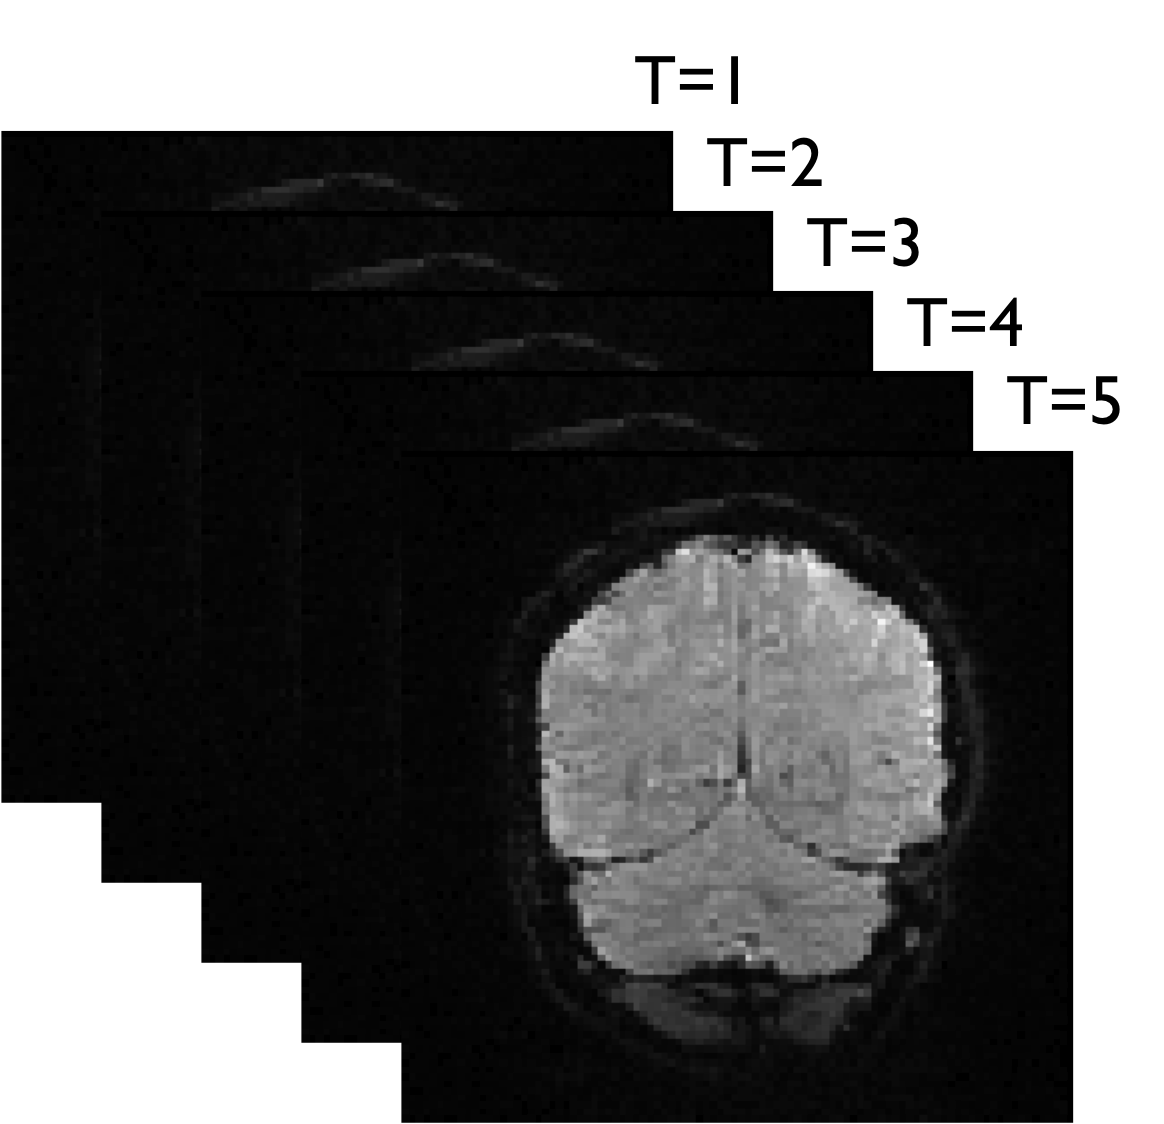
\includegraphics[height=5.7cm]{figures/t1_2_3_4_5}
\end{frame}

\begin{frame}
\frametitle{Time-series in fMRI data}
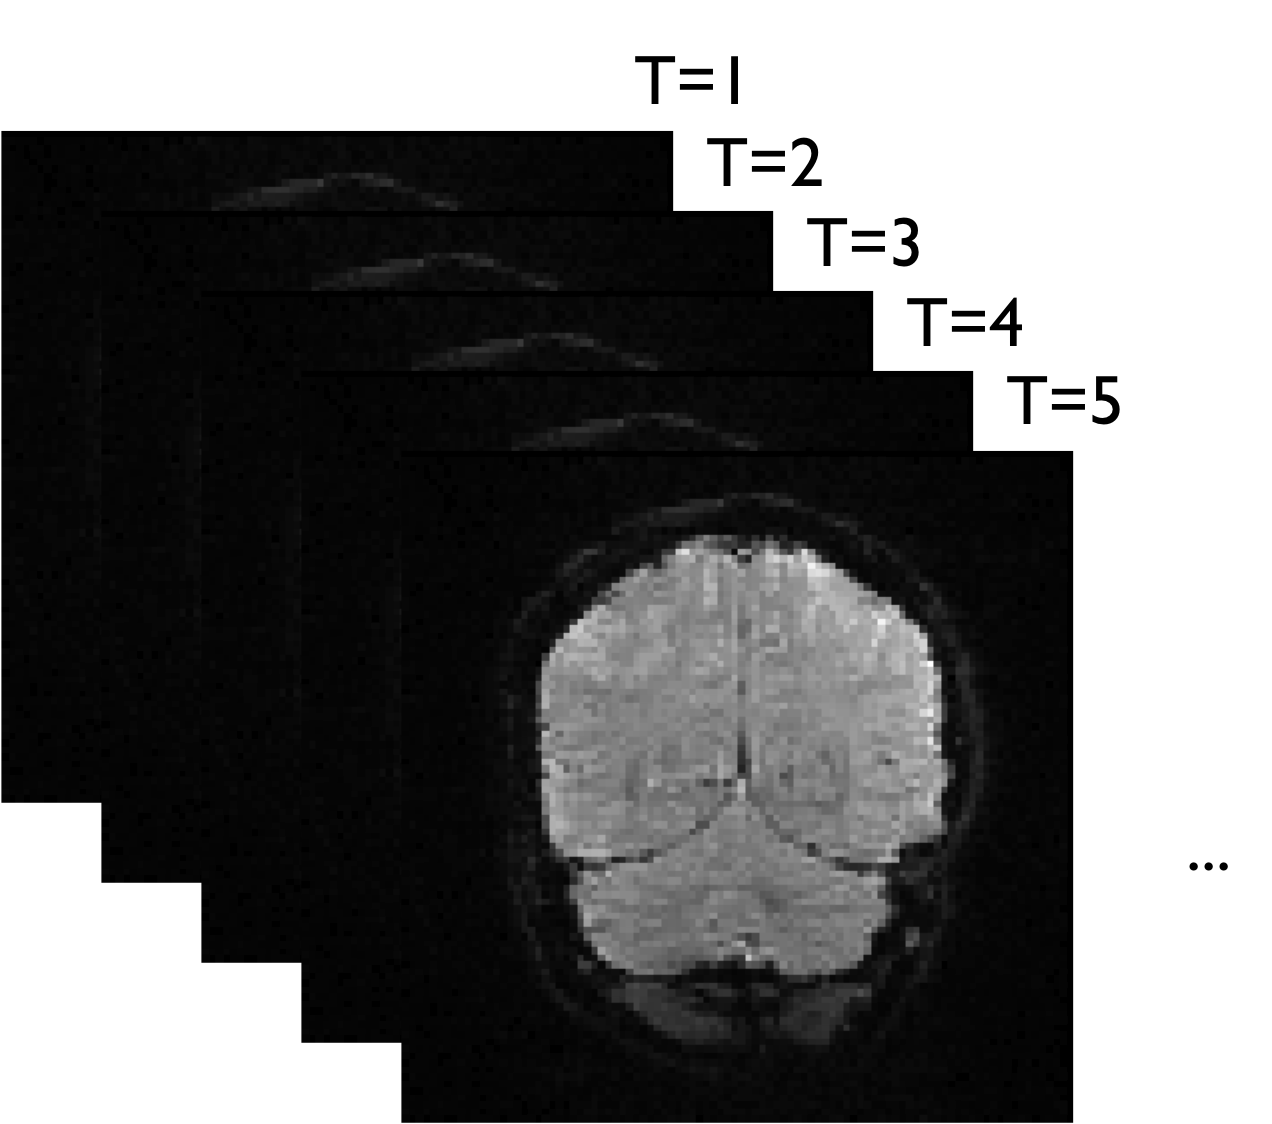
\includegraphics[height=5.7cm]{figures/t1_5_etc}
\end{frame}

\begin{frame}
\frametitle{Time-series in fMRI data}
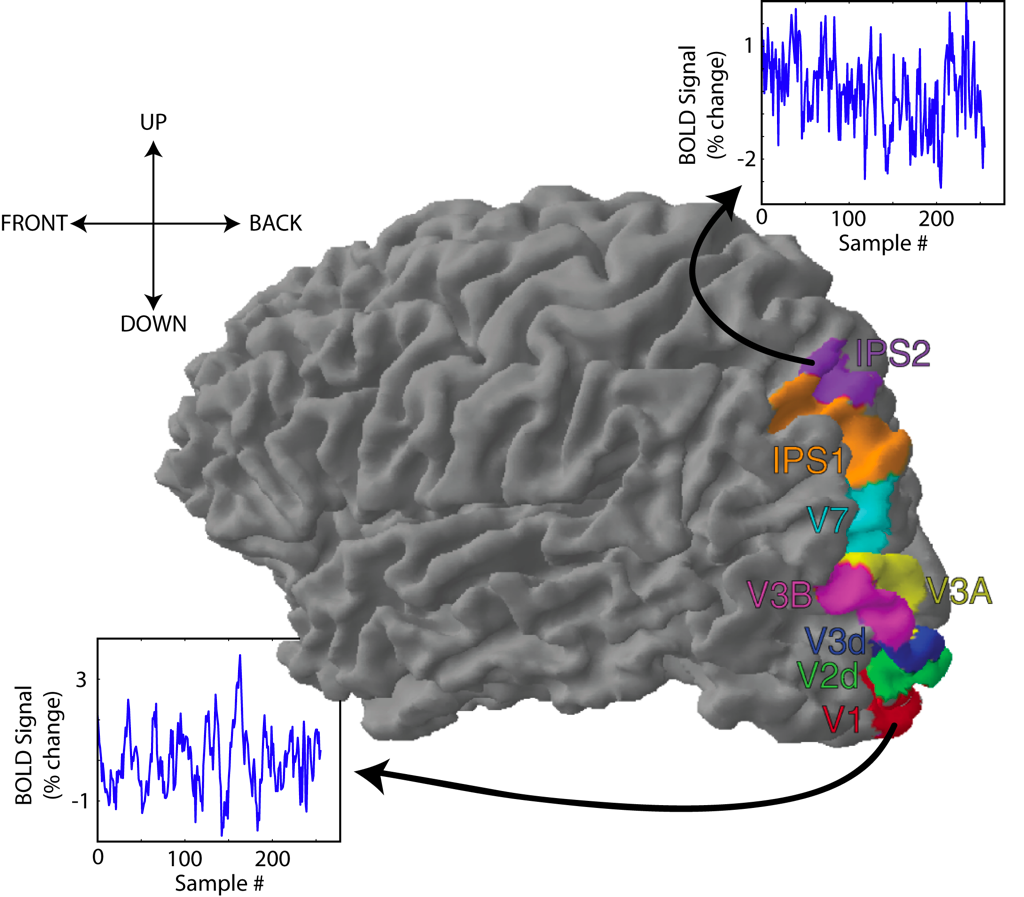
\includegraphics[height=5.7cm]{figures/brain_w_tseries}
\end{frame}

\begin{frame}
\frametitle{Functional connectivity}
What are the functional relations between different parts of the brain?
\end{frame}

\begin{frame}
\frametitle{Resting-state fMRI}
The functional connectivity at 'rest'
\end{frame}

\begin{frame}
\frametitle{Correlations}
\pause
Zero-order correlation:
\pause
$r = \sum_{i=1}^{N}{\frac{(x_i-\hat{x})(y_i-\hat{y})}{\sigma_x \sigma_y}}$
\end{frame}

\begin{frame}
\frametitle{Cross-correlation}
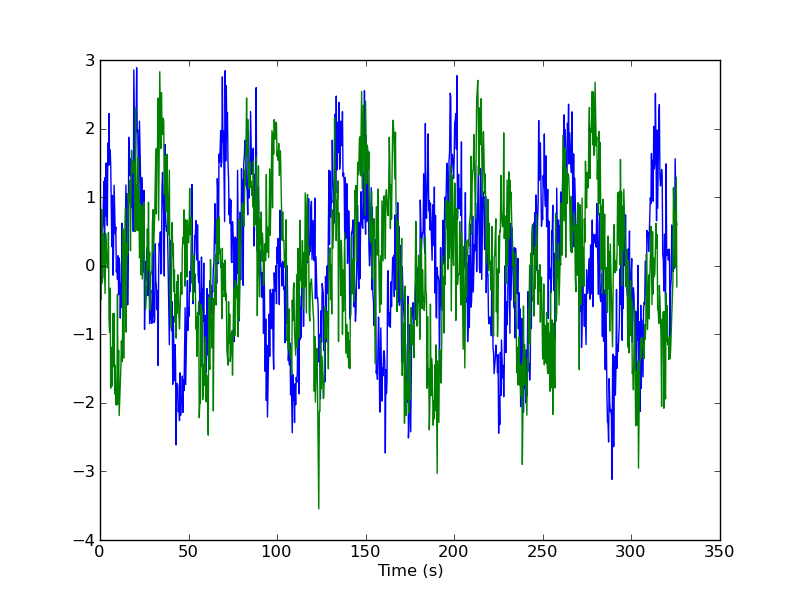
\includegraphics[height=5.7cm]{figures/outa_phase_tseries}
\end{frame}

\begin{frame}
\frametitle{Cross-correlation}
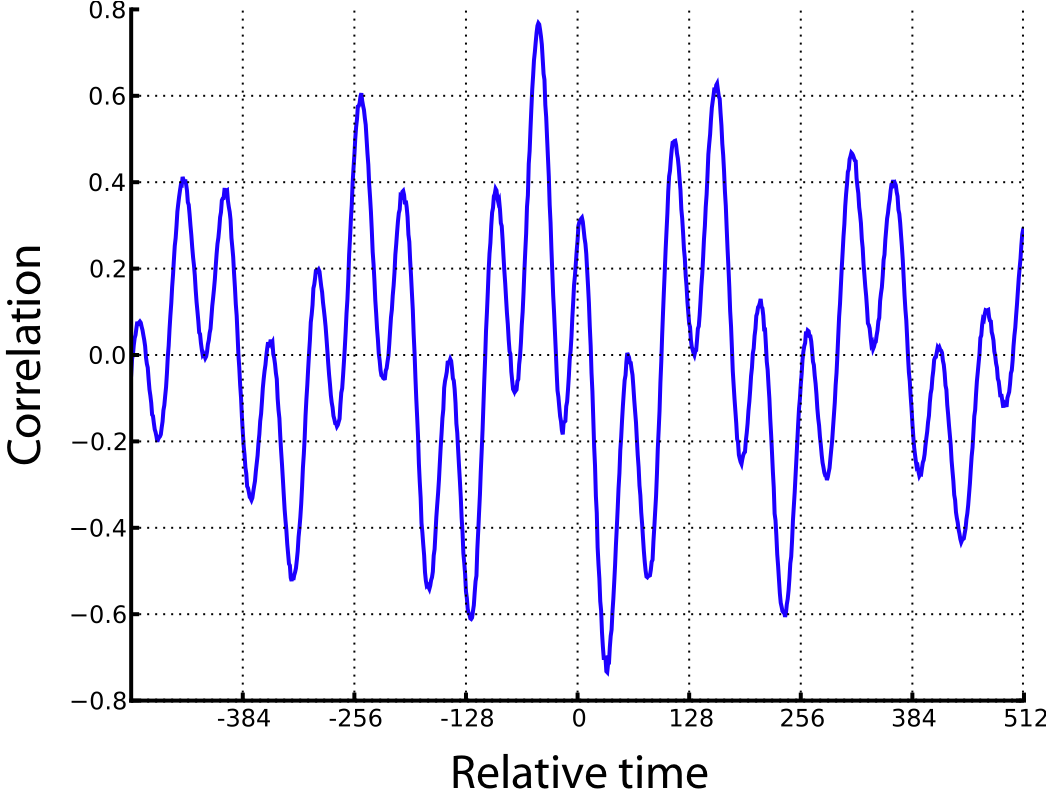
\includegraphics[height=5.7cm]{figures/outa_phase_xcorr}
\end{frame}

\end{document}
